% Copyright 2004 by Till Tantau <tantau@users.sourceforge.net>.
%
% In principle, this file can be redistributed and/or modified under
% the terms of the GNU Public License, version 2.
%
% However, this file is supposed to be a template to be modified
% for your own needs. For this reason, if you use this file as a
% template and not specifically distribute it as part of a another
% package/program, I grant the extra permission to freely copy and
% modify this file as you see fit and even to delete this copyright
% notice. 

\documentclass[aspectratio=169]{beamer}
%\documentclass{beamer}

\setbeamersize{text margin left=10mm, text margin right=10mm}

\defbeamertemplate{headline}{my header}{%
\vskip1pt%sb
\makebox[0pt][l]{\,\insertshortauthor}%
\hspace*{\fill}\insertshorttitle/\insertshortsubtitle\hspace*{\fill}%
\llap{\insertpagenumber/\insertpresentationendpage\,}
}
\setbeamertemplate{headline}[my header]

\usepackage{graphicx}
\usepackage{caption}
\usepackage{subcaption}
\usepackage{soul}
\usepackage{tkz-euclide}
\usetikzlibrary{calc}
\usepackage[]{algorithm2e}
\usepackage{changepage}
\usepackage{amssymb}
\usepackage{xcolor}
\usepackage{mathtools}
\usepackage{tcolorbox}
\usepackage{tikz}
\usetikzlibrary{arrows}
\usepackage{tikz-3dplot}
\usepackage{tkz-euclide}
\usepackage{circuitikz}
\usepackage{pgfplots}
\pgfplotsset{width=7cm,compat=1.8}
\usepackage[outdir=./]{epstopdf}

\usetikzlibrary{positioning}
% \usepackage[math]{cellspace}
% \cellspacetoplimit 4pt
% \cellspacebottomlimit 4pt
%\usetikzlibrary{arrows.meta}
% sqare of half axes
\newcommand{\asa}{3}
\newcommand{\bsa}{1}
\newcommand{\csa}{0.25}
% view angle
\tdplotsetmaincoords{70}{135}

%\setbeamertemplate{itemize items}{-}

%\usepackage{helvet}
\usefonttheme{professionalfonts} % using non standard fonts for beamer
%\usefonttheme{serif} % default family is serif
%\usepackage{fontspec}
%\setmainfont{Liberation Serif}

% There are many different themes available for Beamer. A comprehensive
% list with examples is given here:
% http://deic.uab.es/~iblanes/beamer_gallery/index_by_theme.html
% You can uncomment the themes below if you would like to use a different
% one:
%\usetheme{AnnArbor}
%\usetheme{Antibes}
%\usetheme{Bergen}
%\usetheme{Berkeley}
%\usetheme{Berlin}
%\usetheme{Boadilla}
%\usetheme{boxes}
%\usetheme{CambridgeUS}
%\usetheme{Copenhagen}
%\usetheme{Darmstadt}
%\usetheme{default}
%\usetheme{Frankfurt}
%\usetheme{Goettingen}
%\usetheme{Hannover}
%\usetheme{Ilmenau}
%\usetheme{JuanLesPins}
%\usetheme{Luebeck}
%\usetheme{Madrid}
%\usetheme{Malmoe}
%\usetheme{Marburg}
%\usetheme{Montpellier}
%\usetheme{PaloAlto}
%\usetheme{Pittsburgh}
%\usetheme{Rochester}
%\usetheme{Singapore}
%\usetheme{Szeged}
%\usetheme{Warsaw}

\def\mf{\ensuremath\mathbf}
\def\mb{\ensuremath\mathbb}
\def\lp{\ensuremath\left(}
\def\rp{\ensuremath\right)}
\def\lv{\ensuremath\left\lvert}
\def\rv{\ensuremath\right\rvert}
\def\lV{\ensuremath\left\lVert}
\def\rV{\ensuremath\right\rVert}
\def\lc{\ensuremath\left\{}
\def\rc{\ensuremath\right\}}
\def\ls{\ensuremath\left[}
\def\rs{\ensuremath\right]}
\def\bmx{\ensuremath\begin{bmatrix*}[r]}
\def\emx{\ensuremath\end{bmatrix*}}
\def\bmxc{\ensuremath\begin{bmatrix*}[c]}
% \def\t{\lp t\rp}
% \def\k{\ls k\rs}


\newcommand{\demoex}[2]{\onslide<#1->\begin{color}{black!60} #2 \end{color}}
\newcommand{\demoexc}[3]{\onslide<#1->\begin{color}{#2} #3 \end{color}}
\newcommand{\anim}[3]{\onslide<#1->{\begin{color}{#2!60} #3 \end{color}}}
\newcommand{\ct}[1]{\lp #1\rp}
\newcommand{\dt}[1]{\ls #1\rs}


% \newenvironment{rcases}
% {\left.\begin{aligned}}
% {\end{aligned}\right\rbrace}


\title{Linear Systems}

% A subtitle is optional and this may be deleted
\subtitle{Linear Dynamical Systems: State Space View}

\author{Sivakumar Balasubramanian}
% - Give the names in the same order as the appear in the paper.
% - Use the \inst{?} command only if the authors have different
%   affiliation.

\institute[Christian Medical College] % (optional, but mostly needed)
{
  \inst{}%
  Department of Bioengineering\\
  Christian Medical College, Bagayam\\
  Vellore 632002
}
% - Use the \inst command only if there are several affiliations.
% - Keep it simple, no one is interested in your street address.

\date{}
% - Either use conference name or its abbreviation.
% - Not really informative to the audience, more for people (including
%   yourself) who are reading the slides online

\subject{Lecture notes on linear systems}
% This is only inserted into the PDF information catalog. Can be left
% out. 

% If you have a file called "university-logo-filename.xxx", where xxx
% is a graphic format that can be processed by latex or pdflatex,
% resp., then you can add a logo as follows:

% \pgfdeclareimage[height=0.5cm]{university-logo}{university-logo-filename}
% \logo{\pgfuseimage{university-logo}}

% Delete this, if you do not want the table of contents to pop up at
% the beginning of each subsection:
\AtBeginSubsection[]
{
  \begin{frame}<beamer>{Outline}
    \tableofcontents[currentsection,currentsubsection]
  \end{frame}
}

% Let's get started
\begin{document}

\pgfplotsset{
  compat=1.8,
  colormap={whitered}{color(0cm)=(white); color(1cm)=(orange!75!red)}
}

\begin{frame}
  \titlepage
\end{frame}


\begin{frame}{States of a system}
\begin{itemize}
    \item A characteristic feature of most dynamical systems is their memory, i.e. the system's response (or output) depends on the present and past values of its input; We are only deal with causal systems here.

    \item If we get interested in a system at some arbitrary time $t_0$, we might not have a complete record of the past input to the system.

    \item The idea of a \textit{state} deals with this problem. 

    \item \textbf{Defintion}: \textit{The state $\mf{x}\lp t_0\rp$ of a system is the information at time $t_0$, which along with the input $u\lp t\rp,\, \forall t \geq t_0$ can be used to uniquely determine the system output $y\lp t\rp, \, \forall t \geq t_0$.}

    \item The state $\mf{x}\lp t_0\rp$ summarizes all the information ones needs to know about the system's past in order to predict its future.

    \item Examples of states of a system:
    \begin{itemize}
        \item Position and velocity of a mass acted up by a force.
        \item Capacitor voltage and inductor current of a electrical network.
        \item Initial conditions of a differential equation describing a system.
    \end{itemize}
\end{itemize}
\end{frame}


\begin{frame}{States of a system}
\begin{small}
In general, the state and the input will determine the system's output.
\[ \begin{rcases}
\mf{x}\lp t_0 \rp \\
u\lp t\rp, \,\, \forall t \geq t_0
\end{rcases} \rightarrow y\lp t\rp, \,\, \forall t \geq t_0 \]

In the case of a linear system, if 
\[ \begin{rcases}
\mf{x}_1\lp t_0 \rp \\
u_1\lp t\rp, \,\,\,\, \forall t \geq t_0
\end{rcases} \rightarrow y_1\lp t\rp, \,\, \forall t \geq t_0 \,\, \text{ and }\,\,\,\, 
\begin{rcases}
\mf{x}_2\lp t_0 \rp \\
u_2\lp t\rp, \,\, \forall t \geq t_0
\end{rcases} \rightarrow y_2\lp t\rp, \,\, \forall t \geq t_0
\]

\[ \implies \begin{rcases}
a_1\mf{x}_1\lp t_0 \rp + a_2\mf{x}_2\lp t_0 \rp \\
a_1u_1\lp t\rp + a_2u_2\lp t\rp, \,\, \forall t \geq t_0
\end{rcases} \rightarrow a_1y_1\lp t\rp + a_2y_2\lp t\rp, \,\, \forall t \geq t_0
\]

For a linear system, knowing the system output to the states and the input will allow us to know the complete output.

\begin{itemize}
  \item \textbf{Zero State Response}: $\left. \mf{x}\lp t_0\rp = \mf{0}; \,\, u\lp t\rp, \, t \geq t_0\right\} \rightarrow y_{zs}\lp t\rp, \forall t \geq t_0$
  \item \textbf{Zero Input Response}: $\left. \mf{x}\lp t_0\rp; \,\, u\lp t\rp = 0, \, t \geq t_0\right\} \rightarrow y_{zi}\lp t\rp, \forall t \geq t_0$
\end{itemize}

$y_{zs}\lp t\rp + y_{zi}\lp t\rp$ gives the complete response.
\end{small}
\end{frame}

\begin{frame}{States of a system}

\begin{columns}
\begin{column}{0.3\textwidth}
\begin{tikzpicture}[every node/.style={draw,outer sep=0pt,thick}, scale=0.8]
%define the spring
\tikzstyle{spring}=[thick,decorate,decoration={zigzag,pre length=0.12cm,post length=0.12cm,amplitude=1.3mm,segment length=6}]

%define the dashpot
\tikzstyle{damper}=[thick,decoration={markings,
  mark connection node=dmp,
  mark=at position 0.5 with 
  {
      \node (dmp) [thick,inner sep=0pt,transform shape,rotate=-90,minimum width=15pt,minimum height=3pt,draw=none] {};    
      \draw [thick] ($(dmp.north east)+(2pt,0)$) -- (dmp.south east) -- (dmp.south west) -- ($(dmp.north west)+(2pt,0)$);
      \draw [thick] ($(dmp.north)+(0,-5pt)$) -- ($(dmp.north)+(0,5pt)$);
  }
}, decorate]

%define the spring-dashpot
\tikzstyle{spr-dash}=[thick,decorate,decoration={markings,
  mark connection node=sqr,
  mark=at position 0.5 with
  {
      \node (sqr) [thick,minimum width=16pt,minimum height=24pt,draw=none] {};
      \draw [thick] (sqr.north west) -- (sqr.north east);
      \draw [thick] (sqr.south west) -- (sqr.south east);
      \draw [spring] (sqr.south west) -- (sqr.north west);
      \draw [damper] (sqr.south east) -- (sqr.north east);
  }
  }]

%define the ground
\tikzstyle{ground}=[fill,pattern=north east lines,draw=none,minimum width=0.75cm,minimum height=0.3cm]

\begin{scope}[xshift=5.5cm]
%draw the frame mass
\node (M1) [minimum width=1cm,minimum height=1cm] {$m_1$};
 
%draw the vehicle mass
\node (M2) at (M1.north) [yshift=+1.8cm, minimum width=1cm, minimum height=1cm] {$m_2$};

\node (ground-medium) at (M1.south) [ground,yshift=-1.3cm,minimum width=4cm,anchor=north] {};
\draw (ground-medium.north west) -- (ground-medium.north east);

\draw [spr-dash] (ground-medium.north) -- (M1.south);
\node [draw=none] at ($(ground-medium.north)+(-1cm,0.7cm)$) {$k_{1}$};
\node [draw=none] at ($(ground-medium.north)+(1.1cm,0.7cm)$) {$b_{1}$};
\draw [spr-dash] (M1.north) -- (M2.south);
\node [draw=none] at ($(M1.north)+(-1.0cm,0.7cm)$) {$k_{2}$};
\node [draw=none] at ($(M1.north)+(1.1cm,0.7cm)$) {$b_{2}$};
 
\draw [-latex,thick] (M2.north) ++ (0, 0.5cm) -- (M2.north);
\draw [dashed,thin] (M2.east) ++ (0.5cm, 0) -- +(1.0cm, 0);
\node [draw=none, right] at ($(M2.east) + (1.5cm, 0)$) {$x_{2}$};

\draw [dashed,thin] (M1.west) ++ (-0.5cm, 0) -- +(-1.0cm, 0);
\node [draw=none, left] at ($(M1.west) + (-1.5cm, 0cm)$) {$x_{1}$};

\node [draw=none, yshift=0.7cm] at (M2.north) {$f$};
\end{scope}
\end{tikzpicture}
\end{column}

\begin{column}{0.7\textwidth}
\begin{small}
\begin{itemize}
    \item In the system shown, the input $u\lp t\rp$ is the force $f\lp t\rp$ applied to $m_2$, and the output $y\lp t\rp$ is the position of $m_2$ $\lp x_2\lp t\rp\rp$.

    \item $y\lp t\rp$ depends not only on $f\lp t\rp$, but also on: $\dot{x}_2\lp t\rp$, $x_1\lp t\rp$ and $\dot{x}_1\lp t\rp$.

    \item For the same input $u$, we can obtain different output $y$ if the starting states are different. Thus, knowledge of the states are essential for correctly predicting the behavior of the system.

    \item In general, the dynamics of a system in terms of its states, input(s) and output(s) is mathematically represented as,
    \vspace{-0.2cm}
    \[ \begin{cases} 
    \dot{\mf{x}}\lp t\rp = \mf{f}\lp \mf{x}\lp t\rp, \mf{u}\lp t\rp\rp \rightarrow \text{\textit{State Equation}}\\
    \mf{y}\lp t\rp = \mf{g}\lp \mf{x}\lp t\rp, \mf{u}\lp t\rp\rp \rightarrow \text{\textit{Measurement Equation}}
    \end{cases}
    \]    
    where, $\mf{x} \in \mb{R}^n$, $\mf{u} \in \mb{R}^p$, and $\mf{y} \in \mb{R}^m$, and $t \in \mb{R}$ represents times. 
\end{itemize}
\end{small}
\end{column}
\end{columns}
\end{frame}


\begin{frame}{State space representation of linear systems}
\begin{itemize}
    \item In the case of a linear system, the equations representing the dynamics takes a simpler form,
    \[ \dot{\mf{x}}\ct{t} = \mf{A}\ct{t}\mf{x}\ct{t} + \mf{B}\ct{t}\mf{u}\ct{t} \]
    \[ \mf{y}\ct{t} = \mf{C}\ct{t}\mf{x}\ct{t} + \mf{D}\ct{t}\mf{u}\ct{t} \]
    where, 
    \begin{itemize}
        \item $\mf{A}\ct{t} \in \mb{R}^{n \times n}$ is the \textit{system} matrix.
        \item $\mf{B}\ct{t} \in \mb{R}^{n \times p}$ is the \textit{input} matrix.
        \item $\mf{C}\ct{t} \in \mb{R}^{m \times n}$ is the \textit{output} matrix.
        \item $\mf{D}\ct{t} \in \mb{R}^{m \times p}$ is the \textit{feedforward} matrix.
    \end{itemize}

    \item In the case of time-invariant system, the matrices are constant.
    \[ \dot{\mf{x}}\ct{t} = \mf{A}\mf{x}\ct{t} + \mf{B}\mf{u}\ct{t} \]
    \[ \mf{y}\ct{t} = \mf{C}\mf{x}\ct{t} + \mf{D}\mf{u}\ct{t} \]

    \item These two equations represent how the states and the measured outputs of the system are affected by the current states and inputs. The individual terms in these matrices indicate how a particular state/input affects another state/output.
\end{itemize}
\end{frame}


\begin{frame}{State space representation of linear systems}
\begin{small}
Consider a LTI system represented by the following differential equation,
\[ \ddot{y}\ct{t} + a_1\dot{y}\ct{t} + a_2 y\ct{t} = u\ct{t} \]

We can obtain a state space representation of this differential equation by choosing two states, $x_1\ct{t} = y\ct{t}$ and $x_2\ct{t} = \dot{y}\ct{t}$,
\[ \dot{\mf{x}}\ct{t} = \bmx \dot{x}_1\ct{t}\\ \dot{x}_2\ct{t} \emx = \bmx \dot{y}\ct{t}\\ \ddot{y}\ct{t} \emx = \bmxc x_2\ct{t}\\ -a_2x_1\ct{t} -a_1x_2\ct{t} + u\ct{t} \emx \]  
\[ \dot{\mf{x}}\ct{t} = \bmx 0 & 1 \\ -a_2 & -a_1\emx \mf{x}\ct{t} + \bmx 0 \\ 1\emx \mf{u}\ct{t} \]
\[ \mf{y}\ct{t} = \bmx 1 & 0 \emx \mf{x}\ct{t} \]

The choice of state for a system is not unique. If for a linear system, $\mf{x}\ct{t}$ is a state, then so is $\hat{\mf{x}}\ct{t} = \mf{T}\mf{x}\ct{t}$, where $\mf{T}$ is invertible.

\demoex{2}{
If $\lp \mf{A}, \mf{B}, \mf{C}, \mf{D}\rp$ are the different matrices associated with a LTI system with state $\mf{x}\ct{t}$. Derive the matrcies when $\mf{T}\mf{x}\ct{t}$ is chosen as the state.}
\end{small}
\end{frame}


\begin{frame}{Block diagram representation of linear systems} 
\begin{itemize}
    \item Pictorial representation of different componenets of a system and their  inter-connections can provide insights into the behavior of the system.

    \item Helps breakdown a complex system into a set of simpler systems connected to each other.

    \item Linear systems in general can be built using three basic elements:
\end{itemize}
\begin{center}
    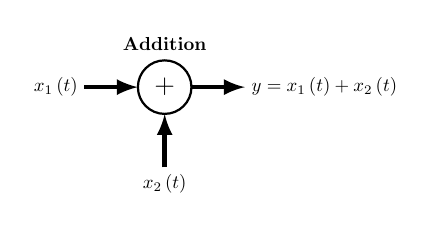
\begin{tikzpicture}[scale=0.68, transform shape]
        \draw[white] (-2.5,-2.1) rectangle ++(7.1,3.2);
        \node[] at (0,0.8) {\textbf{Addition}};
        \draw[thick,black] (0,0) circle (0.5cm);
        \node[] at (0,0) {{\Large $+$}};
        \draw[-latex, ultra thick] (-1.5,0) -- (-0.5, 0);
        \draw[-latex, ultra thick] (0, -1.5) -- (0, -0.5);
        \draw[-latex, ultra thick] (0.5,0) -- (1.5, 0);
        \node[left] at (-1.5, 0) {$x_1\ct{t}$};
        \node[below] at (0, -1.5) {$x_2\ct{t}$};
        \node[right] at (1.5, 0) {$y = x_1\ct{t} + x_2\ct{t}$};
    \end{tikzpicture}
    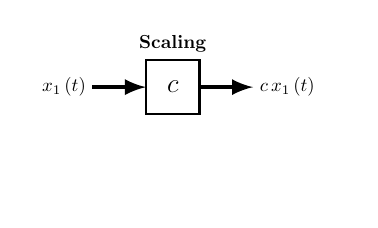
\begin{tikzpicture}[scale=0.68, transform shape]
        \draw[white] (-2.7,-2.1) rectangle ++(6.0,3.2);
        \draw[thick, black] (-0.5,-0.5) rectangle ++(1,1);
        \node[] at (0,0.8) {\textbf{Scaling}};
        \node[] at (0,0) {{\Large $c$}};
        \draw[-latex, ultra thick] (-1.5,0) -- (-0.5, 0);
        \draw[-latex, ultra thick] (0.5,0) -- (1.5, 0);
        \node[left] at (-1.5, 0) {$x_1\ct{t}$};
        \node[right] at (1.5, 0) {$c\,x_1\ct{t}$};
    \end{tikzpicture}
    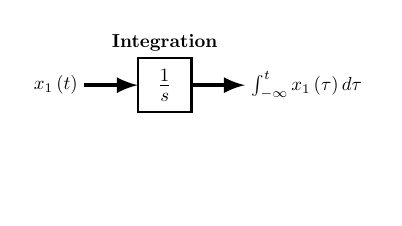
\begin{tikzpicture}[scale=0.68, transform shape]
        \draw[white] (-2.4,-2.1) rectangle ++(6.3,3.1);
        \draw[thick, black] (-0.5,-0.5) rectangle ++(1,1);
        \node[] at (0,0.8) {\textbf{Integration}};
        \node[] at (0,0) {{\Large $\frac{1}{s}$}};
        \draw[-latex, ultra thick] (-1.5,0) -- (-0.5, 0);
        \draw[-latex, ultra thick] (0.5,0) -- (1.5, 0);
        \node[left] at (-1.5, 0) {$x_1\ct{t}$};
        \node[right] at (1.5, 0) {$\int_{-\infty}^tx_1\ct{\tau}d\tau$};
    \end{tikzpicture}
\end{center}

Represent the following linear differential equations using the three elementary block,
\begin{itemize}
    \item $\dot{y}\ct{t} + 0.1y\ct{t} = u\ct{t}$
    \item $\ddot{y}\ct{t} + 2\dot{y}\ct{t} + 5y\ct{t} = u\ct{t} -2 \ddot{u}\ct{t}$
\end{itemize}
\end{frame}


\begin{frame}{State space representation of discrete-time linear systems}

\begin{itemize}
    \item Discrete-time linear system,
    \[ \mf{x}\dt{k+1} = \mf{A}\dt{k}\mf{x}\dt{k} + \mf{B}\dt{k}\mf{u}\dt{k} \]
    \[ \mf{y}\dt{k} = \mf{C}\dt{k}\mf{x}\dt{k} + \mf{D}\dt{k}\mf{u}\dt{k} \]
    where, $k \in \mb{Z}$ correspond to time index.
    \begin{itemize}
        \item $\mf{A}\dt{k} \in \mb{R}^{n \times n}$ is the \textit{system} matrix.
        \item $\mf{B}\dt{k} \in \mb{R}^{n \times p}$ is the \textit{input} matrix.
        \item $\mf{C}\dt{k} \in \mb{R}^{m \times n}$ is the \textit{output} matrix.
        \item $\mf{D}\dt{k} \in \mb{R}^{m \times p}$ is the \textit{feedforward} matrix.
    \end{itemize}

    \item In the case of time-invariant system, the matrices are constant.
    \[ \mf{x}\dt{k+1} = \mf{A}\mf{x}\dt{k} + \mf{B}\mf{u}\dt{k} \]
    \[ \mf{y}\dt{k} = \mf{C}\mf{x}\dt{k} + \mf{D}\mf{u}\dt{k} \]
\end{itemize}
\end{frame}


\begin{frame}{State space representation of discrete-time linear systems}
\begin{small}
Consider a LTI system represented by the following differential equation,
\[ y\dt{k} + a_1y\dt{k-1} + a_2 y\dt{k-2} = u\dt{k} \]

We can obtain a state space representation of this difference equation by choosing two states, $x_1\dt{k} = y\dt{k-1}$ and $x_2\dt{k} = y\dt{k-2}$,
\[ \mf{x}\dt{k+1} = \bmx x_1\dt{k+1}\\ x_2\dt{k+1} \emx = \bmxc y\dt{k}\\ y\dt{k-1} \emx = \bmxc -a_1x_1\dt{k} - a_2x_2\dt{k} + u\dt{k}\\ x_1\dt{k} \emx \]  
\[ \mf{x}\dt{k+1} = \bmx -a_1 & -a_2 \\ 1 & 0\emx \mf{x}\dt{k} + \bmx 1 \\ 0\emx \mf{u}\dt{k} \]
\[ \mf{y}\dt{k} = \bmx -a_1 & -a_2 \emx \mf{x}\dt{k} + \bmx 1 \emx \mf{u}\dt{k} \]

The choice of state for a system is not unique. If for a linear system, $\mf{x}\dt{k}$ is a state, then so is $\hat{\mf{x}}\dt{k} = \mf{T}\mf{x}\dt{k}$, where $\mf{T}$ is invertible.
\end{small}
\end{frame}


\begin{frame}{Block diagram representation of discrete-time linear systems} 
\begin{itemize}
    \item Discrete-time linear systems in general can be built using three basic elements:
\end{itemize}
\begin{center}
    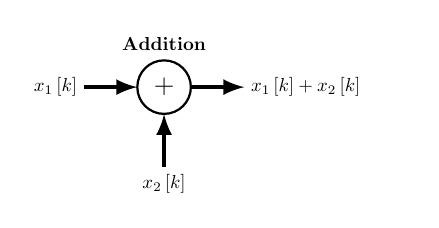
\begin{tikzpicture}[scale=0.68, transform shape]
        \draw[white] (-2.5,-2.1) rectangle ++(7.1,3.2);
        \node[] at (0,0.8) {\textbf{Addition}};
        \draw[thick,black] (0,0) circle (0.5cm);
        \node[] at (0,0) {{\Large $+$}};
        \draw[-latex, ultra thick] (-1.5,0) -- (-0.5, 0);
        \draw[-latex, ultra thick] (0, -1.5) -- (0, -0.5);
        \draw[-latex, ultra thick] (0.5,0) -- (1.5, 0);
        \node[left] at (-1.5, 0) {$x_1\dt{k}$};
        \node[below] at (0, -1.5) {$x_2\dt{k}$};
        \node[right] at (1.5, 0) {$x_1\dt{k} + x_2\dt{k}$};
    \end{tikzpicture}
    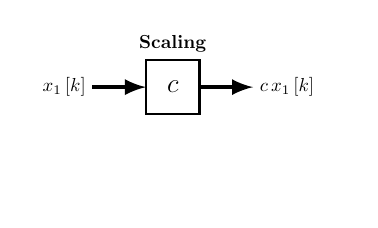
\begin{tikzpicture}[scale=0.68, transform shape]
        \draw[white] (-2.7,-2.1) rectangle ++(6.0,3.2);
        \draw[thick, black] (-0.5,-0.5) rectangle ++(1,1);
        \node[] at (0,0.8) {\textbf{Scaling}};
        \node[] at (0,0) {{\Large $c$}};
        \draw[-latex, ultra thick] (-1.5,0) -- (-0.5, 0);
        \draw[-latex, ultra thick] (0.5,0) -- (1.5, 0);
        \node[left] at (-1.5, 0) {$x_1\dt{k}$};
        \node[right] at (1.5, 0) {$c\,x_1\dt{k}$};
    \end{tikzpicture}
    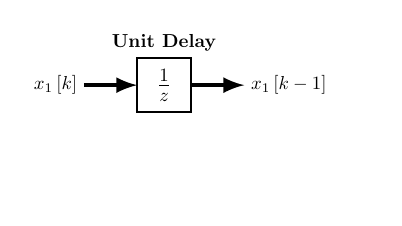
\begin{tikzpicture}[scale=0.68, transform shape]
        \draw[white] (-2.4,-2.1) rectangle ++(6.3,3.1);
        \draw[thick, black] (-0.5,-0.5) rectangle ++(1,1);
        \node[] at (0,0.8) {\textbf{Unit Delay}};
        \node[] at (0,0) {{\Large $\frac{1}{z}$}};
        \draw[-latex, ultra thick] (-1.5,0) -- (-0.5, 0);
        \draw[-latex, ultra thick] (0.5,0) -- (1.5, 0);
        \node[left] at (-1.5, 0) {$x_1\dt{k}$};
        \node[right] at (1.5, 0) {$x_1\dt{k-1}$};
    \end{tikzpicture}
\end{center}

Represent the following linear differential equations using the three elementary block,
\begin{itemize}
    \item $y\dt{k} + 0.1y\dt{k} = u\dt{k}$
    \item $y\dt{k-2} + 2y\dt{k-1} + 5y\dt{k} = u\dt{k} -2 u\dt{k-2}$
    \item $y\dt{k} = \frac{1}{5}\sum_{l=0}^{4} u\dt{k-l}$
\end{itemize}
\end{frame}

\begin{frame}{State space visualization}
\begin{small}
For systems with two states, we can  visualize the state space trajectories of the system to gain better understanding of the system dynamics.

The state dynamics of a mass, spring and damper system is given by the following equation,
\[ \dot{\mf{x}}\ct{t} = \bmx 0 & 1\\ -\frac{k}{m} & -\frac{b}{m}\emx \mf{x}\ct{t} + \bmx 0 \\ \frac{1}{m}\emx \mf{u}\ct{t} \]
\end{small}
\vspace{-0.3cm}
\begin{figure}
    \begin{subfigure}[b]{0.3\textwidth}
        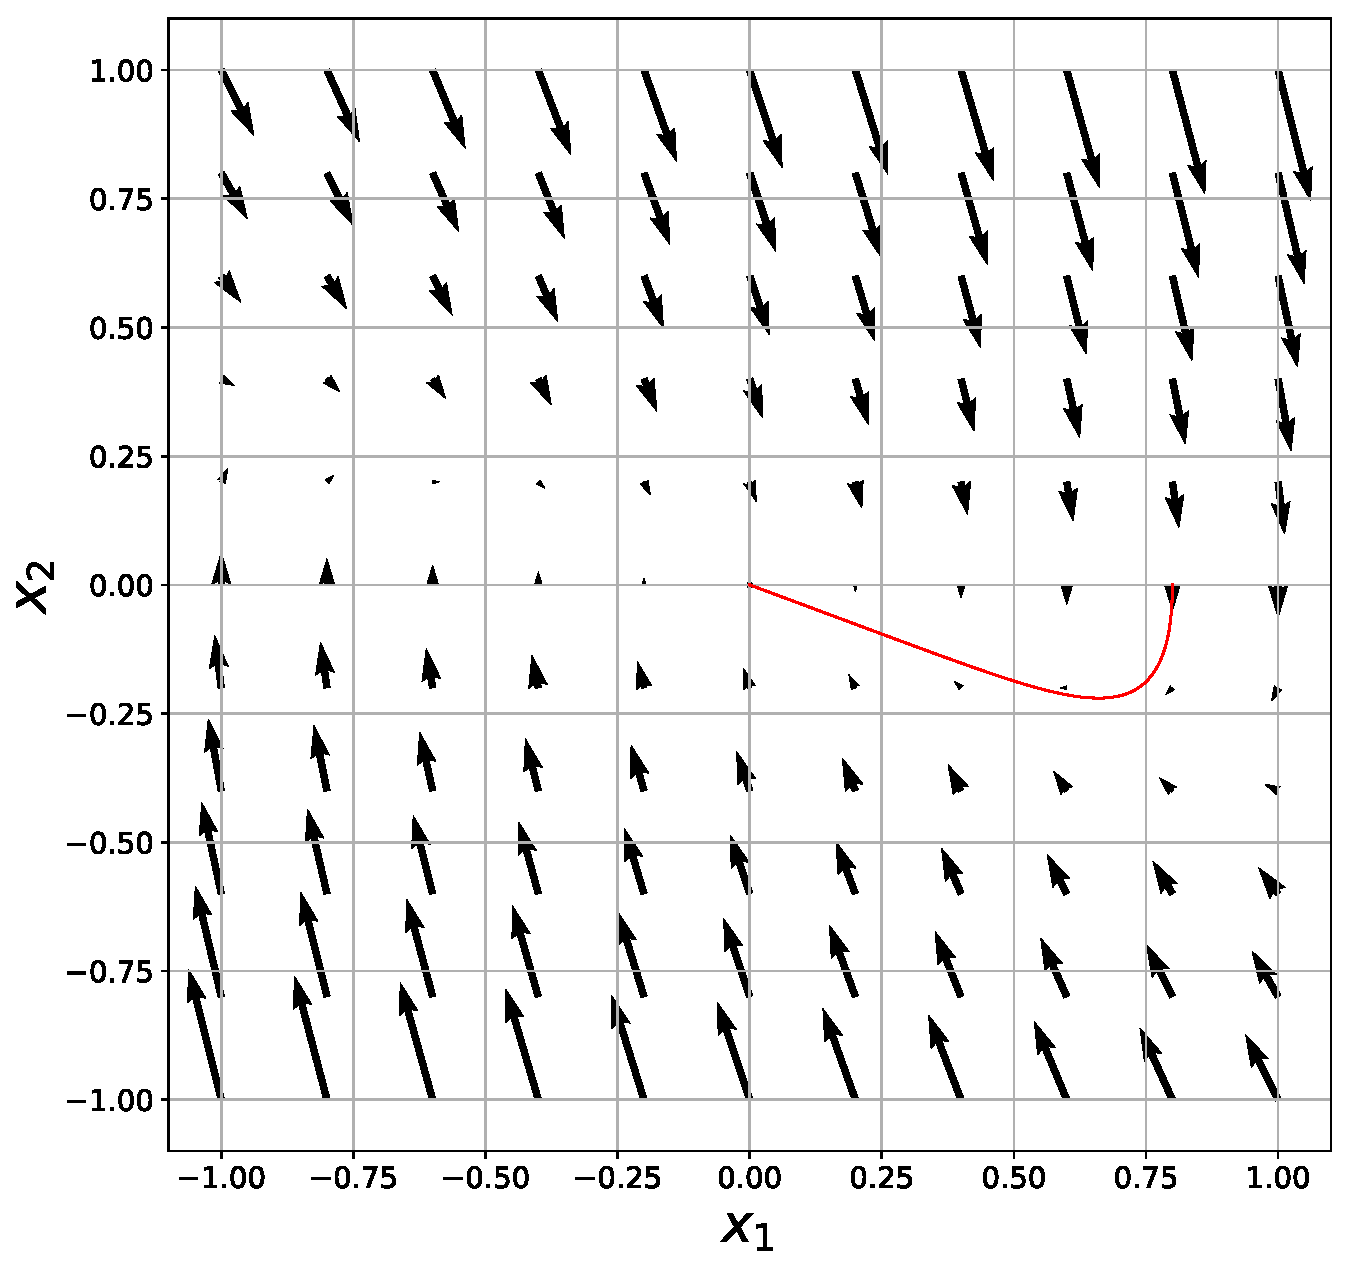
\includegraphics[width=\linewidth]{img/osc2.eps}
        \captionsetup{labelformat=empty}
        \caption{\small $m=1, \, b=3, \, k=1$}
        \label{fig:gull}
    \end{subfigure}\hspace{0.1cm}
    \begin{subfigure}[b]{0.3\textwidth}
        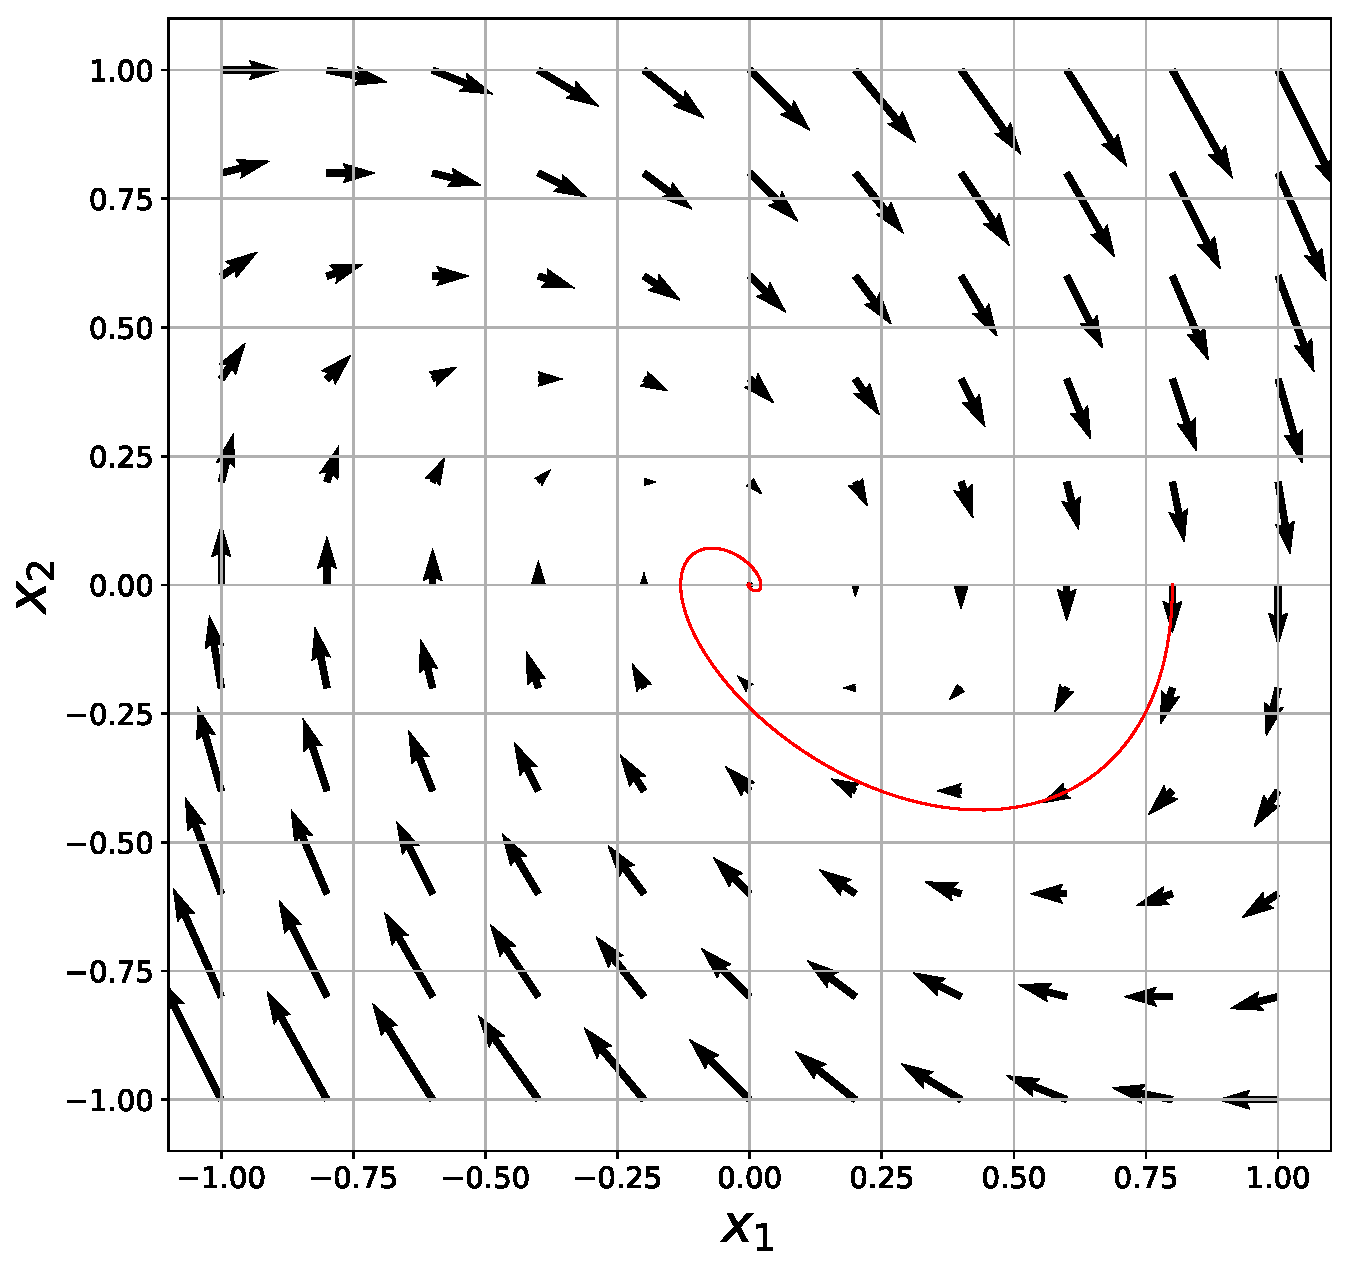
\includegraphics[width=\linewidth]{img/osc1.eps}
        \captionsetup{labelformat=empty}
        \caption{\small $m=1, \, b=1, \, k=1$}
        \label{fig:gull2}
    \end{subfigure}\hspace{0.1cm}
    \begin{subfigure}[b]{0.3\textwidth}
        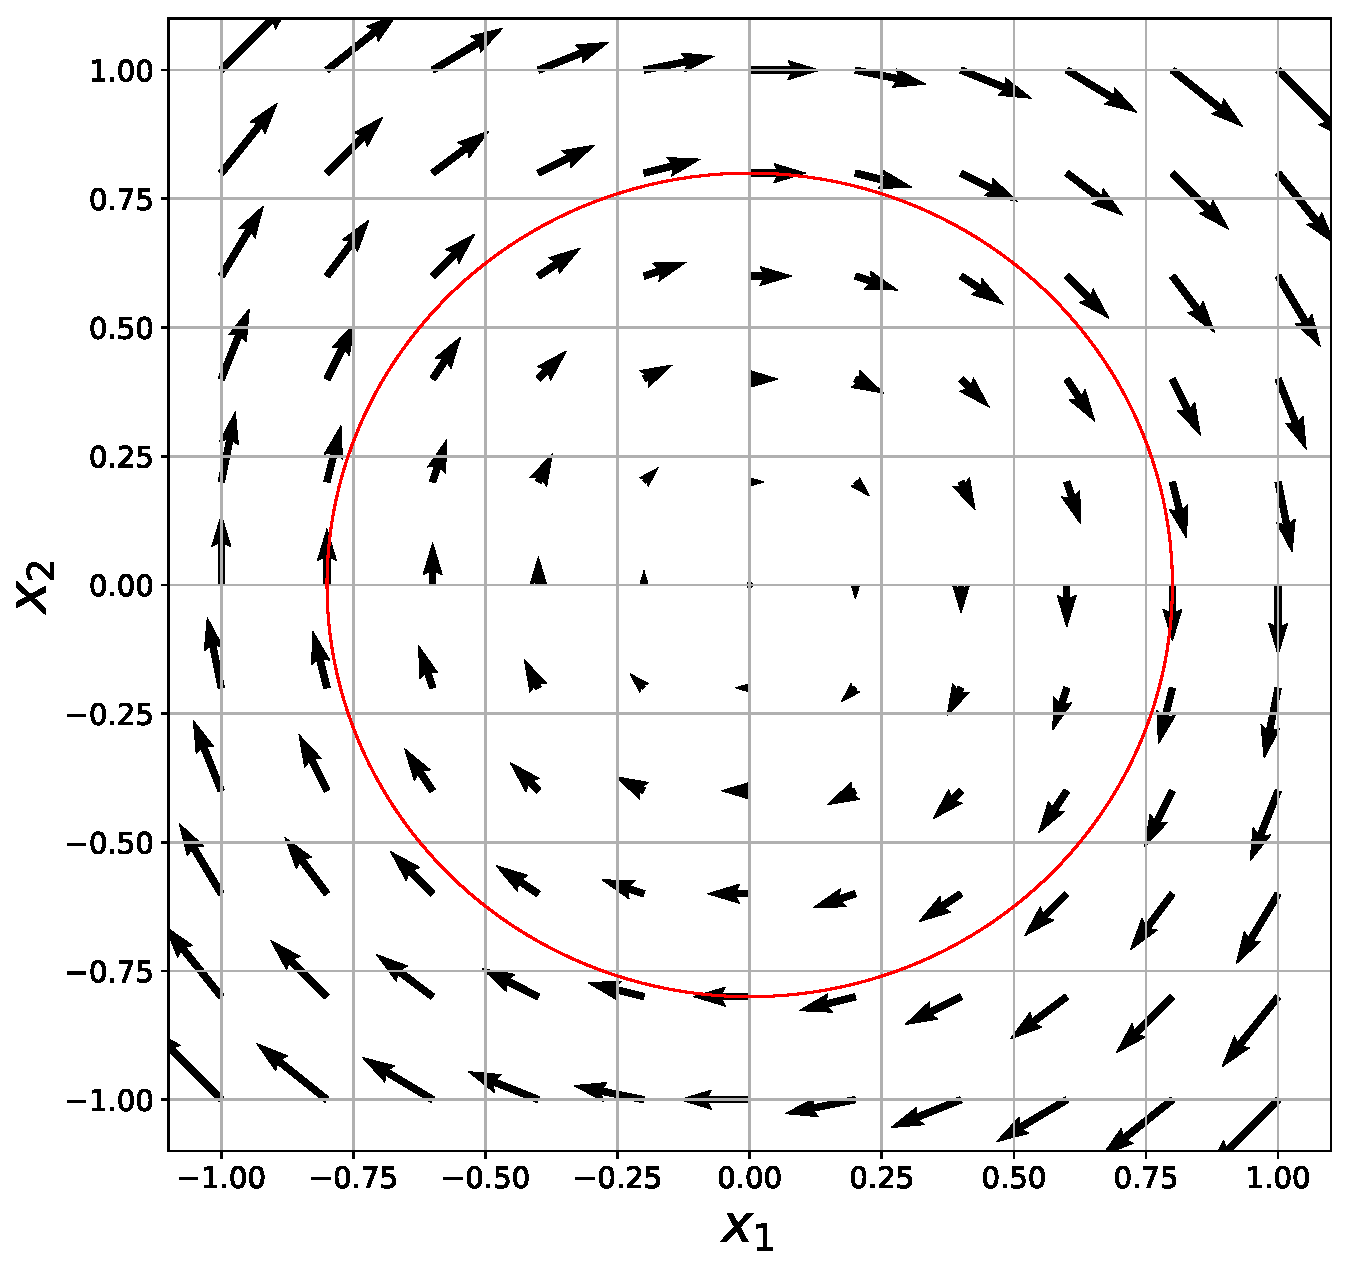
\includegraphics[width=\linewidth]{img/osc.eps}
        \captionsetup{labelformat=empty}
        \caption{\small $m=1, \, b=0, \, k=1$}
        \label{fig:tiger}
    \end{subfigure}%
\end{figure}

\end{frame}

\end{document}